\section{Correlation between Question Hops and Agent Iterations}
\label{appendix_sec:correlation_between_hops_and_agent_iterations}

\begin{figure*}[thbp]
  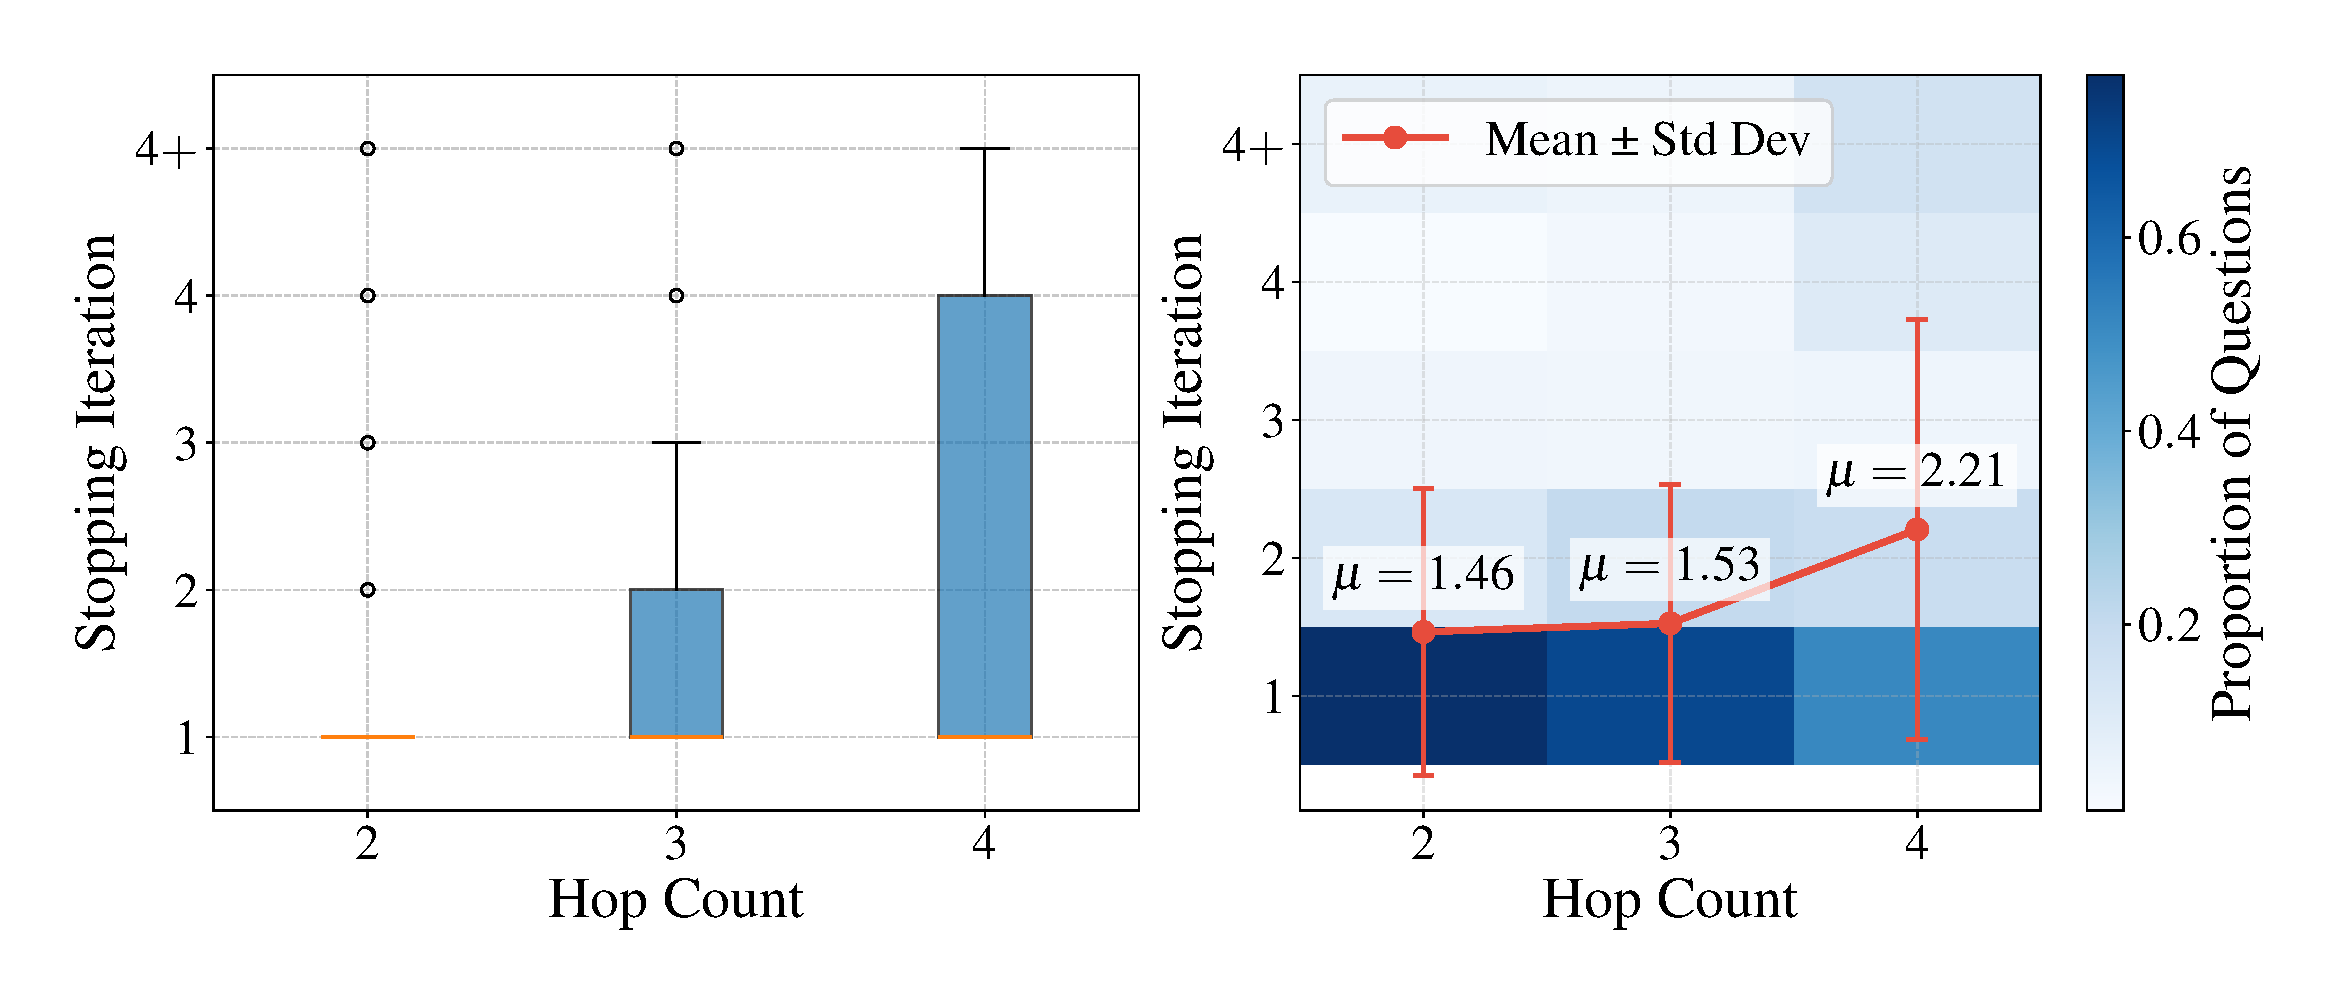
\includegraphics[width=\textwidth]{figures/experiments/hop_vs_agent_iteration_correlation.pdf}
  \caption{Analysis of the relationship between the number of hops in questions and the required number of agent iterations on the MuSiQue dataset. For each hop count, we analyse the number of iterations required by \gear to determine question answerability. The maximum iteration limit was set to 4, with ``4+'' indicating cases where the agent could not determine answerability within this limit. The visualization presents two complementary perspectives on the same data: the left panel shows a box plot emphasizing the median and distribution of stopping iterations, while the right panel focuses on the mean number of iterations across different hop counts.}
  \label{fig:hop_vs_agent_iteration_correlation}
\end{figure*}

The left panel in Figure \ref{fig:hop_vs_agent_iteration_correlation} demonstrates that the median stopping iteration remains consistently at 1 across all hop counts. Additionally, the upper quartile shows a clear upward trend as the number of hops increases. This suggests greater variability in processing time for more complex questions. The right panel illustrates two concurrent trends: as the question hop count increases, the number of questions in the dataset decreases, and the mean number of iterations \gear requires to determine question answerability increases. This pattern indicates that higher-hop questions not only appear less frequently but also typically demand more computational effort to process.
